\documentclass{article}

\usepackage{fancyhdr}
\usepackage{extramarks}
\usepackage{amsmath}
\usepackage{amsthm}
\usepackage{amsfonts}
\usepackage{tikz}
\usepackage[plain]{algorithm}
\usepackage{algpseudocode}
\usepackage{parskip}
\usepackage{enumerate}
\usetikzlibrary{arrows,shapes,positioning,shadows,trees}

%
% Basic Document Settings
%

\topmargin=-0.45in
\evensidemargin=0in
\oddsidemargin=0in
\textwidth=6.5in
\textheight=9.0in
\headsep=0.25in

\linespread{1.1}

\pagestyle{fancy}
\lhead{\hmwkAuthorName}
\chead{\hmwkClass\ (\hmwkClassInstructor): \hmwkTitle}
\rhead{\firstxmark}
\lfoot{\lastxmark}
\cfoot{\thepage}

\renewcommand\headrulewidth{0.4pt}
\renewcommand\footrulewidth{0.4pt}

\setlength\parindent{0pt}

\tikzset{
  basic/.style  = {draw, font=\sffamily, rectangle},
  root/.style   = {basic, rounded corners=2pt, thin, align=center},
  level 2/.style = {basic, rounded corners=6pt, thin,align=center,text width=8em},
  level 3/.style = {basic, thin, align=left, text width=6.5em}
}

%
% Create Problem Sections
%

\newcommand{\enterProblemHeader}[1]{
    \nobreak\extramarks{}{Problem \arabic{#1} continued on next page\ldots}\nobreak{}
    \nobreak\extramarks{Problem \arabic{#1} (continued)}{Problem \arabic{#1} continued on next page\ldots}\nobreak{}
}

\newcommand{\exitProblemHeader}[1]{
    \nobreak\extramarks{Problem \arabic{#1} (continued)}{Problem \arabic{#1} continued on next page\ldots}\nobreak{}
    \stepcounter{#1}
    \nobreak\extramarks{Problem \arabic{#1}}{}\nobreak{}
}

\setcounter{secnumdepth}{0}
\newcounter{partCounter}
\newcounter{homeworkProblemCounter}
\setcounter{homeworkProblemCounter}{1}
\nobreak\extramarks{Problem \arabic{homeworkProblemCounter}}{}\nobreak{}

%
% Homework Problem Environment
%
% This environment takes an optional argument. When given, it will adjust the
% problem counter. This is useful for when the problems given for your
% assignment aren't sequential. See the last 3 problems of this template for an
% example.
%
\newenvironment{homeworkProblem}[1][-1]{
    \ifnum#1>0
        \setcounter{homeworkProblemCounter}{#1}
    \fi
    \section{Problem \arabic{homeworkProblemCounter}}
    \setcounter{partCounter}{1}
    \enterProblemHeader{homeworkProblemCounter}
}{
    \exitProblemHeader{homeworkProblemCounter}
}

%
% Homework Details
%   - Title
%   - Due date
%   - Class
%   - Section/Time
%   - Instructor
%   - Author
%

\newcommand{\hmwkTitle}{Homework\ \#4}
\newcommand{\hmwkDueDate}{February 26, 2015}
\newcommand{\hmwkClass}{CS350 - Algorithms}
\newcommand{\hmwkClassInstructor}{for Professor Andrew Black}
\newcommand{\hmwkAuthorName}{Kristina Frye}

%
% Title Page
%

\title{
    \vspace{2in}
    \textmd{\textbf{\hmwkClass:\ \hmwkTitle}}\\
    \normalsize\vspace{0.1in}\small{Due\ on\ \hmwkDueDate}\\
    \vspace{0.1in}\large{\textit{\hmwkClassInstructor}}
    \vspace{3in}
}

\author{\textbf{\hmwkAuthorName}}
\date{}

\renewcommand{\part}[1]{\textbf{\large Part \Alph{partCounter}}\stepcounter{partCounter}\\}

%
% Various Helper Commands
%

% Useful for algorithms
\newcommand{\alg}[1]{\textsc{\bfseries \footnotesize #1}}

% For derivatives
\newcommand{\deriv}[1]{\frac{\mathrm{d}}{\mathrm{d}x} (#1)}

% For partial derivatives
\newcommand{\pderiv}[2]{\frac{\partial}{\partial #1} (#2)}

% Integral dx
\newcommand{\dx}{\mathrm{d}x}

% Alias for the Solution section header
\newcommand{\solution}{\textbf{\large Solution}}

% Probability commands: Expectation, Variance, Covariance, Bias
\newcommand{\E}{\mathrm{E}}
\newcommand{\Var}{\mathrm{Var}}
\newcommand{\Cov}{\mathrm{Cov}}
\newcommand{\Bias}{\mathrm{Bias}}

\begin{document}

\maketitle

\pagebreak

\begin{homeworkProblem}
    \textbf{Proof of Master Theorem.} Complete the proof, started in class, for the two cases of the 	
    Master Theorem where $a = b^d$ and $a > b^d$\\
    \\
    \textbf{Master Theorem:} Let $T(n) = a T(\frac{n}{b}) + f(n)$. If $f(n) \in \Theta(n^d)$ where $d\ge0$
    in recurrence, then
    \[
    	T(n) \in 
    		\begin{cases}
			\Theta(n^d) & \text{ if } a < b^d\\
			\Theta(n^d \log{n}) & \text{ if } a = b^d\\
			\Theta(n^{log_ba}) & \text{ if } a>b^d
		\end{cases}
    \]
    
    \textbf{Proof:}\\
    Solve for $T(n):$
    \begin{align*}
    	T\left(\frac{n}{b}\right) &= a \cdot T\left(\frac{n}{b^2}\right) + f\left(\frac{n}{b}\right) \\
	\implies T(n) &= a \left(a \cdot T\left(\frac{n}{b^2}\right) + f\left(\frac{n}{b}\right)\right) + f(n)\\
	\implies T(n) &= a^2 \cdot T\left(\frac{n}{b^2}\right) + a \cdot f\left(\frac{n}{b}\right) + f(n)\\
	\implies T(n) &= a^k \cdot T\left(\frac{n}{b^k}\right) + \sum_{i=0}^{k-1}a^i f\left(\frac{n}{b^i}\right)
    \end{align*}
    If $n=b^k$, then:
    \[
    	T(n) = a^{\log_bn} \cdot T(1) + \sum_{i=0}^{\log_bn}a^i f\left(\frac{n}{b^i}\right)
    \]
    We know that $f(n) \in \Theta(n^d)$ and $a^{\log_bn} = n^{\log_ba}$, so:
    \[
    	T(n) = n^{\log_ba} + \sum_{i=0}^{\log_bn}a^i c \left(\frac{n}{b^i}\right)^d
    \] for some constant $c$. Therefore:
    \[
    	T(n) = n^{\log_ba} + \sum_{i=0}^{\log_bn}c \cdot n^d \left(\frac{a}{b^{d}}\right)^i
	 = n^{\log_ba} + c \cdot n^d\sum_{i=0}^{\log_bn} \left(\frac{a}{b^{d}}\right)^i
    \]
    \textbf{Case 1 ($a < b^d$)} was proved in class. \textbf{Case 2 ($a = b^d$):} \\
    If $a = b^d$, then $\log_ba = \log_bb^d = d \log_bb = d$. Therefore $n^{\log_ba} = n^d$. So: \\
    \[
    	T(n) = n^d + c \cdot n^d\sum_{i=0}^{\log_bn} 1 = \Theta(n^d \log_bn)
    \]
    \textbf{Case 3 ($a > b^d$):}
    \[
    	T(n) =n^{\log_ba} + c \cdot n^d\sum_{i=0}^{\log_bn} \left(\frac{a}{b^{d}}\right)^i
    \]
    Since $a > b^d$, the last term of the summation will be the largest. By the theorem in the 
    book on page 56, the efficiency class is equal to the largest efficiency class in the summation. 
    Therefore:
    \begin{align*}
    	T(n) &\in max\left \{\Theta\left(n^{\log_ba}\right), 
		\Theta\left(n^d \left(\frac{a}{b^d}\right)^{\log_bn}\right)\right \}\\
	   	&\in max\left \{\Theta\left(n^{\log_ba}\right),
		\Theta\left(n^d \left(\frac{a^{\log_bn}}{b^{d\log_bn}}\right)\right)\right \}\\
		&\in max\left \{\Theta\left(n^{\log_ba}\right),
		\Theta\left(n^d \left(\frac{n^{\log_ba}}{n^{\log_bb^d}}\right)\right)\right \}\\
		&\in max\left \{\Theta\left(n^{\log_ba}\right),
		\Theta\left(n^d \left(\frac{n^{\log_ba}}{n^d}\right)\right)\right \}\\
		&\in max\left \{\Theta\left(n^{\log_ba}\right),
		\Theta\left(n^{\log_ba}\right)\right\}\\
		&\in \Theta\left(n^{\log_ba}\right)
    \end{align*}
    
\end{homeworkProblem}

\begin{homeworkProblem}
    {\bf Application of Master Theorem. } Use the Master Theorem to find the order of growth for the solutions of the following recurrences:
    \begin{enumerate}[(a)]
    	\item $T(n) = 4T\left(\frac{n}{2}\right) + n, T(1) = 1 \implies a = 4, b = 2, d = 1
	\implies b^d = 2 \implies a > b^d \implies \\
	T(n) \in \Theta(n^{\log_24}) 
	\implies T(n) \in \Theta(n^2)$
    	\item $T(n) = 4T\left(\frac{n}{2}\right) + n^2, T(1) = 1 \implies a = 4, b = 2, d = 2
	\implies b^d = 4 \implies a = b^d \implies \\
	T(n) \in \Theta(n^2 \log n)$
    	\item $T(n) = 4T\left(\frac{n}{2}\right) + n^3, T(1) = 1 \implies a = 4, b = 2, d = 3
	\implies b^d = 8 \implies a < b^d \implies \\
	T(n) \in \Theta(n^3)$
    \end{enumerate}
\end{homeworkProblem} 

\begin{homeworkProblem}
	{\bf Quicksort. } 
	\begin{enumerate}[(a)]
		\item Apply Quicksort, by hand, to sort the letters of the word ALGORITHM into
		alphabetical order. Draw the tree of the recursive calls that the algorithm makes,
		marking on the tree the values of $l$ (the index of the left end of the sub-array),
		$r$ (the index of the right end) and $s$ (the index of the pivot after the partition)
		for each of the calls. For the purpose of this exercise only, assume that the first
		element of the sub-array, $A[l]$, is the pivot.
		
		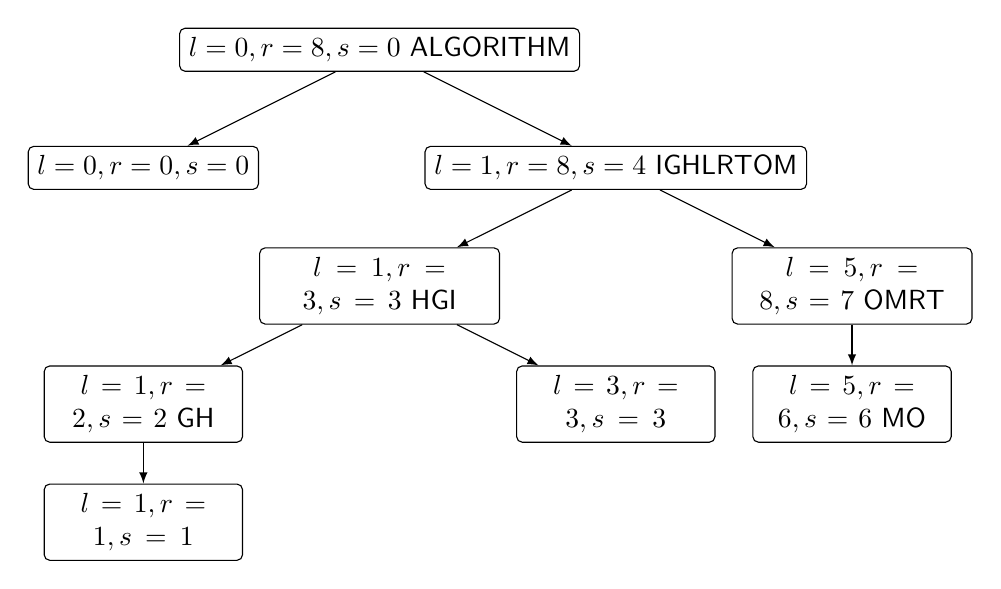
\begin{tikzpicture}[
  		level 1/.style={sibling distance=60mm},edge from parent/.style={->,draw},>=latex]
  			\begin{scope}[every node/.style={root}]
				\node {$l = 0, r=8, s=0$ ALGORITHM}
				child {node {$l=0, r=0, s=0$}}
  				child {node {$l=1,r=8,s=4$ IGHLRTOM}
					child {node {$l=1,r=3,s=3$ HGI}
						child {node {$l=1,r=2,s=2$ GH}
							child {node {$l=1,r=1,s=1$}}}
						child {node {$l=3,r=3,s=3$}}}
					child {node {$l=5,r=8,s=7$ OMRT}
						child {node {$l=5,r=6,s=6$ MO}}}};
			\end{scope}
		\end{tikzpicture}
		\\Result = AGHILMORT
		
		\textbf{Details:}\\
		Partition: ALGORITHM\\
		Input: $l = 0, r = 8, p = A$\\
		$i = 1, j = 9$\\
		$i = 1, A[i] = L > A$\\
		$j = 8..0, A[0] = A \le A$\\
		$swap(A[0], A[0])$\\
		$swap(A[0], A[0])$\\
		$swap(A[0], A[0])$\\
		return $0$\\
		\\
		Partition: LGORITHM\\	
		Input: $l = 1, r=8, p = L$\\
		$i = 1, j=9$\\
		$i = 1..3, A[3] = O > L$\\
		$j = 8..7, A[7] = H \le L$\\
		$swap([A[3], A[7])$\\
		LGHRITOM\\
		$i = 4, A[4] = R > L$\\
		$j = 6..5, A[5] = I \le L$\\
		$swap([A[4], A[5])$\\
		LGHIRTOM\\
		$i = 5, A[5] = R > L$\\
		$j = 4, A[4] = I \le L$\\
		$swap([A[5], A[4])$\\
		LGHRITOM\\
		$5 > 4$\\
		$swap([A[5], A[4])$\\
		LGHIRTOM\\
		$swap([A[1], A[4])$\\
		IGHLRTOM\\
		return $4$\\
		\\
		Partition: IGH\\
		Input: $l = 1, r = 3, p = I$\\
		$i = 1, j = 4$\\
		$i = 2..3, A[3] = H < I$\\
		$j = 3, A[3] = H < I$\\
		$swap(A[3], A[3])$\\
		$3 \ge 3$\\
		$swap(A[3], A[3])$\\
		$swap(A[1], A[3])$\\
		HGI\\
		return $4$\\
		\\
		Partition: HG\\
		Input: $l = 1, r = 2, p = H$\\
		$i = 1, j = 3$\\
		$i = 2, A[2] = G < H$\\
		$j = 2, A[2] = G < H$\\
		$swap(A[2], A[2])$\\
		$2 \ge 2$\\
		$swap(A[2], A[2])$\\
		$swap(A[1], A[2])$\\
		HG\\
		return $2$\\
		\\
		Partition: RTOM\\
		Input: $l = 5, r=8, p = R$\\
		$i = 5, j = 9$\\
		$i = 6, A[6] = T > R$\\
		$j = 8, A[8] =  M < R$\\
		$swap(A[6], A[8])$\\
		RMOT\\
		$i = 8, A[8] = T > R$\\
		$j = 7, A[7] = O < R$\\
		$swap(A[8], A[7])$\\
		RMTO\\
		$8 > 7$\\
		$swap(A[8], A[7])$\\
		RMOT\\
		$swap(A[5], A[7])$\\
		OMRT\\
		return $7$\\
		
		Partition: OM\\
		Input: $l = 5, r = 6, p = O$\\
		$i = 5, j = 7$\\
		$i = 6, A[6] = M < O$\\
		$j = 6, A[6] = M < O$\\
		$swap(A[6], A[6])$\\
		$6 \ge 6$\\
		$swap(A[6], A[6])$\\
		$swap(A[5], A[6])$\\
		MO\\
		return 6\\
		\\
		\item Should an implementation of Quicksort use the first element of a sub-array for
		the pivot? Explain why, or why not.
		\\
		\\
		\textbf{Answer:} The pivot should normally be a random element in the array. If each of the 
		items in the array in random order, then it's okay to choose the first element. However, in 	
		many cases, the array will already have some sort of sorting. In that case, a random 
		element of the array should be chosen instead of the first element, which has a higher 
		probability of being a lower element of the sorted array.
	\end{enumerate}
\end{homeworkProblem}

\begin{homeworkProblem}
	\textbf{Trees.} Prove that Vertex $u$ is an ancestor of vertex $v$ in a rooted ordered tree $T$ if
	and only if $preorder(u) \le preorder(v) \wedge postorder(u) \ge postorder(v)$,
	where $preorder(x)$ and $postorder(x)$ are the numbers assigned to vertex $x$ by the
	preorder and postorder traversals of $T$
	
	\textbf{Proof:}\\
	\textbf{Left $\implies$ Right}\\
	Suppose Vertex $u$ is an ancestor of vertex $v$ in a rooted ordered tree $T$. Then, 
	according to the definition of preorder traversal (Section 5.3 in the book), the root is
	visited before the left and right subtrees are visited (in that order). Therefore, the ancestor
	will be visited before the descendants, which implies that $preorder(u) \le preorder(v)$. 
	During postorder traversal, the root is visited after visiting the left and right subtrees (in
	that order). Therefore, the ancestor will be visited after the descendants, which implies
	that $postorder(u) \ge preorder(v)$
	
	\textbf{Right $\implies$ Left}\\
	Suppose $preorder(u) \le preorder(v) \wedge postorder(u) \ge postorder(v)$ and suppose
	$u$ is not an ancestor of $v$. If $preorder(u) \le preorder(v)$, then $u$ is visited before $v$ in 
	the preorder traversal. This occurs in two cases: $u$ is an ancestor of $v$ or $u$ is in a left 
	branch of the tree and $v$ is in a right branch since the left branch is visited before the right 
	branch in a preorder traversal. Since we are assuming $u$ is not an ancestor of $v$, then
	$u$ must be in the left branch and $v$ must be in the right branch.
	
	Now consider $postorder(u) \ge postorder(v)$. This occurs in two cases: $u$ is an ancestor of 
	$v$, or $u$ is in the right branch of the tree and $v$ is in left branch since, similar to the 
	preorder traversal, the left branch is visited before the right branch in a postorder travel. 
	Since we are assuming $u$ is not an ancestor of $v$, then $u$ must be in the right 
	branch and $v$ is in the left branch. But this contradicts with the earlier finding that 
	$u$ must be in the left branch and $v$ must be in the right branch if $u$ is not a
	ancestor of $v$. Therefore our assumption must be wrong and $u$ must be an
	ancestor of $v$.
	
\end{homeworkProblem}

\begin{homeworkProblem}
	\textbf{Horspool's Algorithm.} Consider the problem of searching for genes in DNA sequences
	using Horspool?s algorithm. A DNA sequence is represented by a text on
	the alphabet ${A, C, G, T}$; the gene or gene segment is the pattern.

	\begin{enumerate}[(a)] 
		\item Construct the shift table for the following gene segment of your chromosome 10: 
			TCCTATTCTT
			\begin{tabular}{| c | c | c | c |}
				\hline
				A & C & G & T\\ \hline
				5 & 2 & 10 & 1\\
				\hline
			\end{tabular}
		\item Apply Horspool's algorithm by hand to locate the above pattern in the following
			DNA sequence:\\
			TTATAGATCTCGTATTCTTTTATAGATCTCCTATTCTT\\
			Your answer should draw each alignment of the pattern and the text, and indicate
			which characters are compared in that alignment.
			\begin{align*}
				\text{TTATAGAT}&\text{\underline{CT}CGTATTCTTTTATAGATCTCCTATTCTT}\\
				\text{TCCTATTC}&\text{\underline{TT} \textit{ (shift by 1)}}
			\end{align*}
			\begin{align*}
				\text{TTATAGATCT}&\text{\underline{C}GTATTCTTTTATAGATCTCCTATTCTT}\\
				\text{TCCTATTCT}&\text{\underline{T} \textit{ (shift by 2)}}
			\end{align*}
			\begin{align*}
				\text{TTATAGATCTC}&\text{\underline{GT}ATTCTTTTATAGATCTCCTATTCTT}\\
				\text{TCCTATTC}&\text{\underline{TT} \textit{ (shift by 1)}}
			\end{align*}
			\begin{align*}
				\text{TTATAGATCTCGT}&\text{\underline{A}TTCTTTTATAGATCTCCTATTCTT}\\
				\text{TCCTATTCT}&\text{\underline{T} \textit{ (shift by 5)}}
			\end{align*}
			\begin{align*}
				\text{TTATAGATCTC}&\text{\underline{GTATTCTT}TTATAGATCTCCTATTCTT}\\
				\text{TC}&\text{\underline{CTATTCTT} \textit{ (shift by 1)}}
			\end{align*}
			\begin{align*}
				\text{TTATAGATCTCGTATTC}&\text{\underline{TTT}TATAGATCTCCTATTCTT}\\
				\text{TCCTATT}&\text{\underline{CTT} \textit{ (shift by 1)}}
			\end{align*}
			\begin{align*}
				\text{TTATAGATCTCGTATTCT}&\text{\underline{TTT}ATAGATCTCCTATTCTT}\\
				\text{TCCTATT}&\text{\underline{CTT} \textit{ (shift by 1)}}
			\end{align*}
			\begin{align*}
				\text{TTATAGATCTCGTATTCTTTT}&\text{\underline{A}TAGATCTCCTATTCTT}\\
				\text{TCCTATTCT}&\text{\underline{T} \textit{ (shift by 5)}}
			\end{align*}
			\begin{align*}
				\text{TTATAGATCTCGTATTCTTTTATAGA}&\text{\underline{T}CTCCTATTCTT}\\
				\text{TCCTATTCT}&\text{\underline{T} \textit{ (shift by 1)}}
			\end{align*}
			\begin{align*}
				\text{TTATAGATCTCGTATTCTTTTATAGAT}&\text{\underline{C}TCCTATTCTT}\\
				\text{TCCTATTCT}&\text{\underline{T} \textit{ (shift by 2)}}
			\end{align*}
			\begin{align*}
				\text{TTATAGATCTCGTATTCTTTTATAGATCT}&\text{\underline{C}CTATTCTT}\\
				\text{TCCTATTCT}&\text{\underline{T} \textit{ (shift by 2)}}
			\end{align*}
			\begin{align*}
				\text{TTATAGATCTCGTATTCTTTTATAGATCTC}&\text{\underline{CT}ATTCTT}\\
				\text{TCCTATTC}&\text{\underline{TT}\textit{ (shift by 1)}}
			\end{align*}
			\begin{align*}
				\text{TTATAGATCTCGTATTCTTTTATAGATCTCCT}&\text{\underline{A}TTCTT}\\
				\text{TCCTATTCT}&\text{\underline{T}\textit{ (shift by 5)}}
			\end{align*}
			\begin{align*}
				\text{TTATAGATCTCGTATTCTTTTATAGATC}&\text{\underline{TCCTATTCTT}}\\
				&\text{\underline{TCCTATTCTT}\textit{ (match!)}}
			\end{align*}
	\end{enumerate}
\end{homeworkProblem}

\begin{homeworkProblem}
	Open Hashing for the input $30, 20, 56, 75, 31, 19$ and hash function $h(K)=K\bmod{11}$
	
	\begin{enumerate}[(a)]
		\item construct the open hash table (draw it).\\
		\begin{tabular}{| l | c | c | c | c | c | c |}
			\hline
			keys & 30 & 20 & 56 & 75 & 31 & 19\\ \hline
			hash addresses & 8   & 9   & 1   &  9  & 9  & 8\\
			\hline
		\end{tabular}
		
		\begin{tabular}{| c | c | c | c | c | c | c | c | c | c | c |}
				\hline
				0 & 1 & 2 & 3 & 4 & 5 & 6 & 7 & 8 & 9 & 10\\ \hline
				  & $\downarrow$ & & & & & & & $\downarrow$ & $\downarrow$ &\\
				  & 56& &   &  &   &   &  & 30&20 & -\\
				   &    &     &    &   &    &    &    & $\downarrow$ & $\downarrow$ & \\
				  &   &   &   & & &  &    & 19 & 75 & -\\
				&    &     &    &   &    &    &    &     & $\downarrow$ & \\
				  &   &   &   &  &  &  &    &   & 31 & \\
				  \hline
			\end{tabular}
		\item find the largest number of key comparisons in a successful search in this table.\\
		\textbf{Answer:} 3
		\item find the average number of key comparisons in a successful search in this table.\\
		\textbf{Answer:} $(1 + 1 + 2 + 1 + 2 + 3) / 6 = 1.67$
	\end{enumerate}
\end{homeworkProblem}

\begin{homeworkProblem}
	Closed hashing for the input $30, 20, 56, 75, 31, 19$ and hash function $h(K) = K \bmod{11}$
	
	\begin{enumerate}
		\item construct the closed hash table (draw it).\\
			\begin{tabular}{| l | c | c | c | c | c | c |}
				\hline
				keys & 30 & 20 & 56 & 75 & 31 & 19\\ \hline
				hash addresses & 8   & 9   & 1   &  9  & 9  & 8\\
				\hline
			\end{tabular}
			
			\begin{tabular}{| c | c | c | c | c | c | c | c | c | c | c |}
				\hline
				0 & 1 & 2 & 3 & 4 & 5 & 6 & 7 & 8 & 9 & 10\\ \hline
				31 & 56 & 19 &    &     &    &    &    &30&20& 75\\
				\hline
			\end{tabular}
		
		\item find the largest number of key comparisons in a successful search in this table.\\
		\textbf{Answer:} 3
		\item find the average number of key comparisons in a successful search in this table.\\
		\textbf{Answer:} $(1 + 1 + 1 + 2 + 3 + 6) / 6 = 2.33$
	\end{enumerate}
\end{homeworkProblem}

\begin{homeworkProblem}
	\textbf{Unique Elements}
	\begin{enumerate}[(a)]
		\item Design an algorithm that uses hashing to check whether all elements of a list
			are distinct.
			
			\begin{algorithmic}
				\Procedure{AreElementsUnique?}{$A[0..n-1]$}\Comment{An array of elements}
					\For{$i = 1 \text{ to } n-1$}
						\State $index \gets GetHashIndex(A[i])$
						\Comment{Get the hash index for the current object}
						\State $t \gets GetHash(index)$ 
						\Comment{Get the pointer to the hash table at index $val$}
						\While{$t \ne null$}
							\If{$t.val = A[i]$}
							\Comment{If the pointer isn't null, check for equality}
								\State \textbf{return false}
								\Comment{This item already exists!}
							\EndIf
							\State $t = t.next$ 
							\Comment{Get the next item in the linked list}
						\EndWhile
						\State $PutHash(val, t)$
						\Comment{Put the value $t$ in the hash table at index $val$}
					\EndFor
					\State \textbf{return true}
					\Comment{No duplicates have been found}
				\EndProcedure
			\end{algorithmic}
			
		\item What is the asymptotic efficiency of your algorithm?\\
		\textbf{Answer:} If you have an extremely bad hash table that maps everything to the 
		same hash index, then you will need to check each value against every other
		value that has already been placed into the table. This is going to be $O(n^2)$
		efficiency. However, if you have a reasonable hash table that only requires a constant
		(average) number of lookups for each value, the efficiency class is $O(n)$.
		
		\item How does it compare with the algorithm in which we first presort the list, and
			then compare adjacent elements?\\
		\textbf{Answer:} If the sorting algorithm used is $O(n \log n)$, then the total efficiency for
		that algorithm is $O(n) + O(n \log n) = O(n \log n)$. This means our hashing
		algorithm is better (as long as we have a good hash function).
	\end{enumerate}
\end{homeworkProblem}

\end{document}
